\documentclass[a4paper]{article}
\usepackage[utf8]{inputenc}

\usepackage[spanish, es-tabla, es-nodecimaldot]{babel}

\usepackage[total={6in, 9in}]{geometry}
\usepackage{amsmath}
%\usepackage{amsfonts}
%\usepackage{amssymb}
\usepackage{graphicx}

\usepackage{hyperref}



\begin{document}

\section{Remuestreo} \label{sec:remuestreo}

En esta secci\'on, analizaremos los efectos del muestreo instant\'aneo en una se\~nal AM. La misma es de la forma:

\begin{equation}
	X_C(t) = \frac{\mathrm{A}_\mathrm{MAX}}{2} \cdot 
	\left(  \frac{1}{2} \cdot \cos{\left( 2\pi \cdot(f_p-f_m) \cdot t\right)} +
	\cos{\left( 2\pi f_p\cdot t\right)} +
	\frac{1}{2} \cdot \cos{\left( 2\pi \cdot (f_p+f_m)\cdot t\right)}
	\right)
\end{equation}

En este caso, se utiliz\'o $f_p=1$kHz y $f_m=100$Hz.  

Para lograr el muestreo instant\'aneo, primero se pasa la se\~nal por el sample and hold. Luego, se la vuelve a muestrear, pero esta vez con la llave anal\'ogica, de manera tal que a la salida se anule la totalidad del tiempo de sample y se conserve s\'olo el de hold. Idealmente, esto es equivalente a multiplicar la se\~nal por un tren de deltas (muestreo ideal), y luego convolucionar con un pulso.
\footnote{Dependiendo de la bibliograf\'ia, puede encontrarse que a esto lo llama ``muestreo flat top'', mientras que con muestreo instant\'aneo se refiere al caso de producto con tren de deltas.}
Gr\'aficamente, donde hab\'ia deltas se obtienen pulsos con el ancho del pulso original y la altura del delta que se reemplaza. 


\begin{figure}[htb]
	\centering
	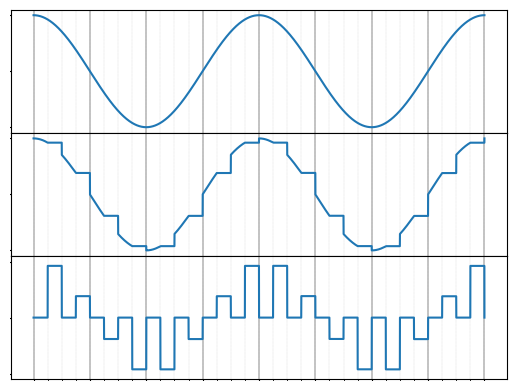
\includegraphics[width=0.8\textwidth]{muestreo_inst.png}
	\caption{Efecto en una se\~nal de entrada (arriba) de pasar primero por un sample and hold (centro), y luego por la llave anal\'ogica (abajo), considerando todo ideal.}
	\label{fig:muestreo_inst}
\end{figure}

Si bien en el caso ideal basta con abrir la llave la totalidad del tiempo que el S\&H est\'a en hold y viceversa, al tener en cuenta las limitaciones de los integrados surgen otras consideraciones. A fines de garantizar que la se\~nal se mantenga lo m\'as constante posible en cada muestra, se quiere evitar que a la salida se observe el tiempo de establecimiento del sample and hold. Por lo tanto, se decidi\'o usar en las mediciones un duty levemente menor para la llave que para el S\&H.

En cuanto al duty cycle de estas mediciones, cuanto m\'as tiempo est\'e abierta la llave, m\'as potencia se recuperar\'a a la salida. 
Sin embargo, hay que tener en cuenta que el S\&H debe estar en hold por m\'as tiempo que la llave est\'a abierta por lo anteriormente discutido, pero si esto se lleva al extremo es posible que el integrado no llegue a seguir a la se\~nal en sample y la salida no sea correcta. 

Considerando que la m\'axima frecuencia que entra en el sistema por $X_C$ es $f_p+f_m=1.1$kHz, por Nyquist la frecuencia de sampleo debe ser mayor a 2.2kHz, y se decidi\'o establecerla en 3kHz, obteni\'endose un per\'iodo de 167$\mu$s. Por otro lado, sabemos por las mediciones realizadas en el LF398 que el tiempo de adquisici\'on del mismo es de 8$\mu$s, pero dejando un margen de error establecemos que no queremos un tiempo de sample inferior a 16$\mu$s. Se obtiene, entonces, que el S\&H debe estar en sample el 9.6\% del tiempo, y por lo tanto se toma 90\% de duty cycle para la llave anal\'ogica. 

Se procedi\'o, pues a realizar mediciones en las condiciones ya mencionadas, a saber: sin el filtro antialiasing, con el sample and hold y la llave anal\'ogica, con $f_s=3$kHz, y un duty cycle del 90\%. Las mismas se observan en las figuras \ref{fig:ej7_llave} y \ref{fig:ej7_out}, que son la salida del sistema sin y con el filtro recuperador respectivamente, con $X_C$ en la entrada.

\begin{figure}[htp]
	\centering
	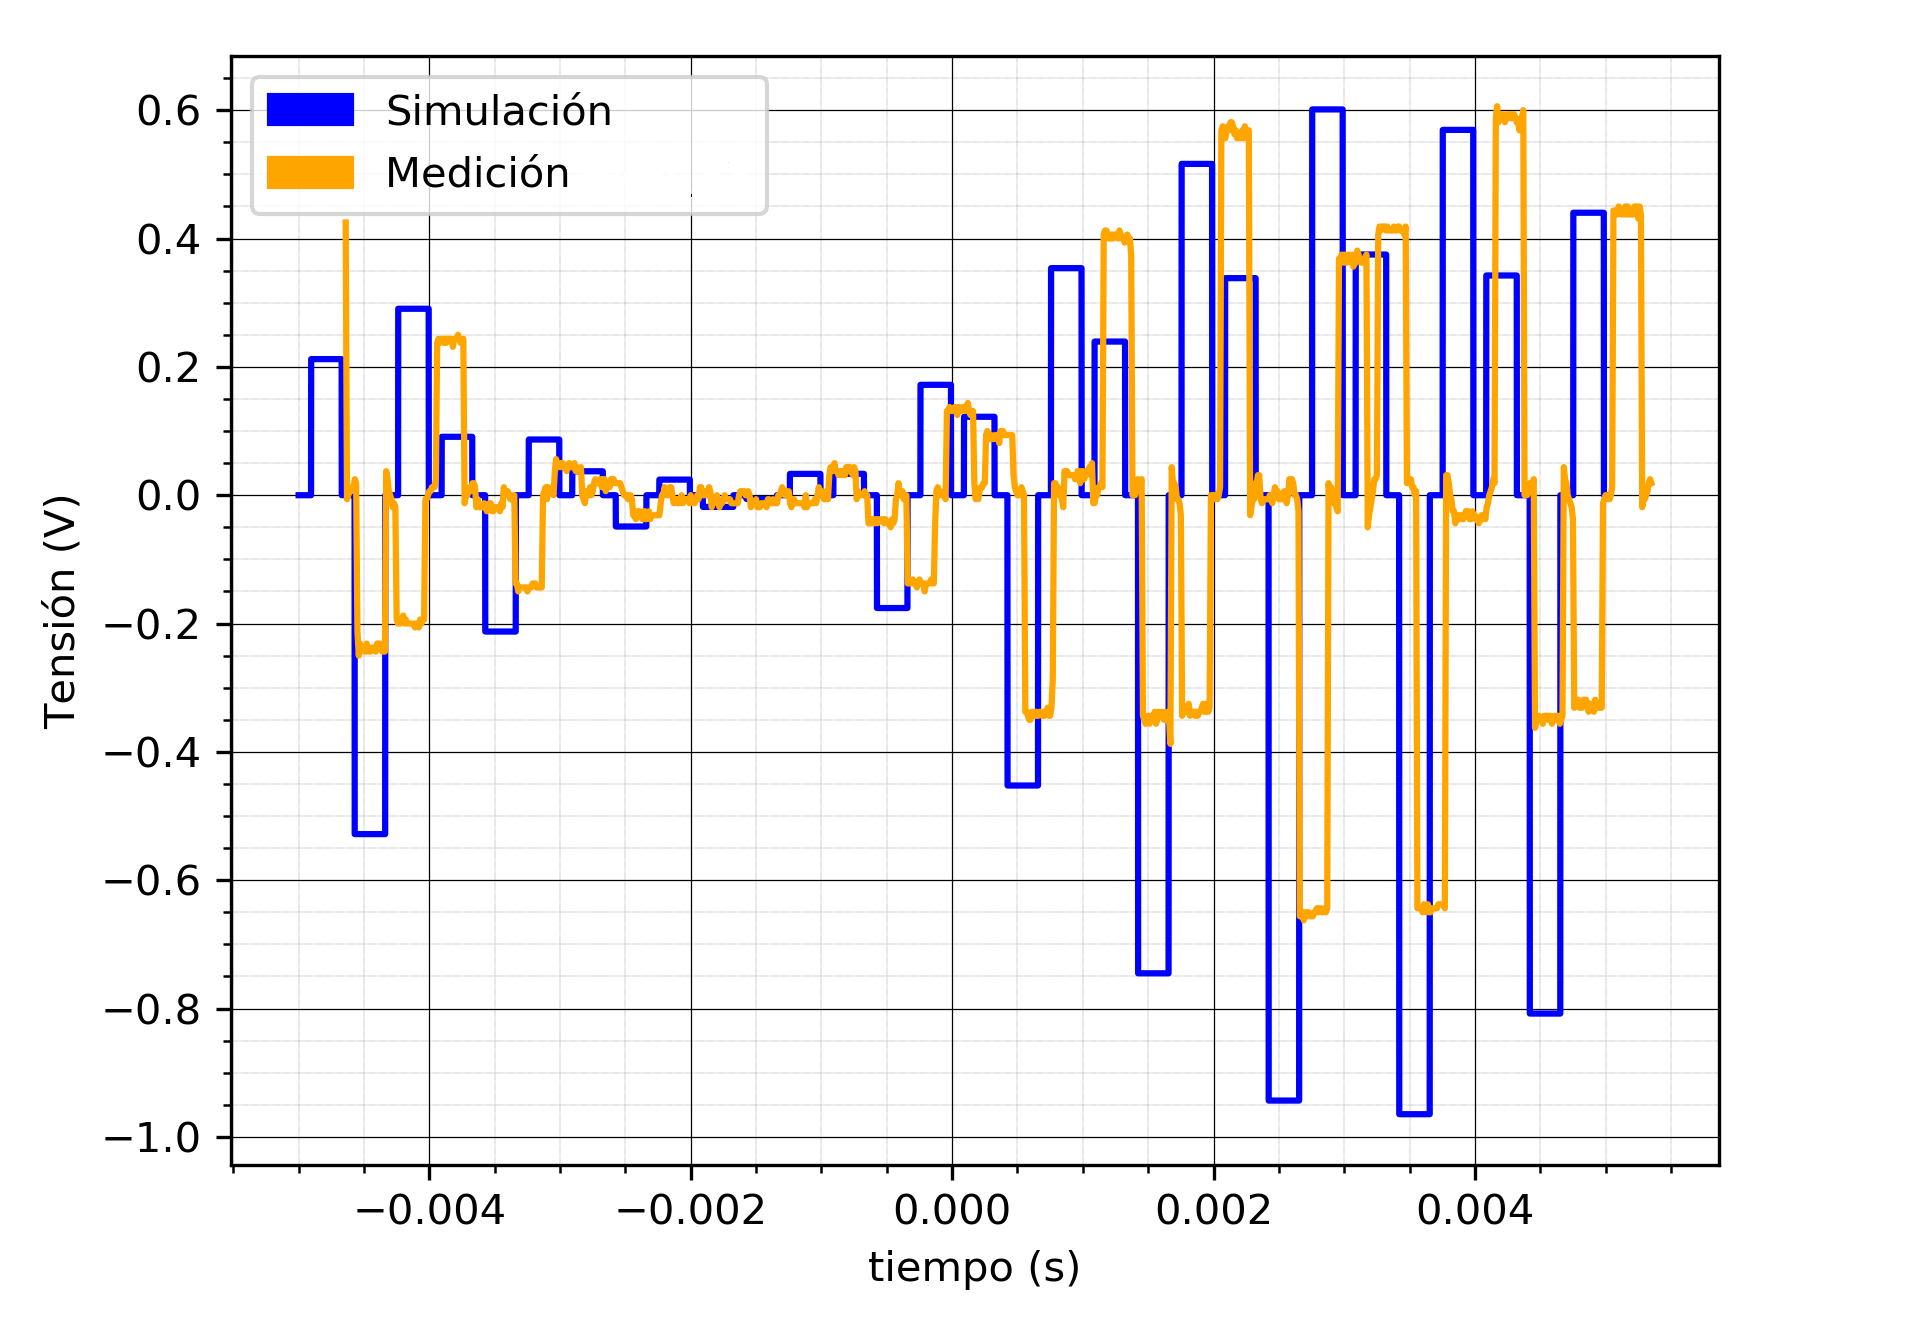
\includegraphics[width=0.7\textwidth]{ej7_meds/med_21.png}
	\caption{Se\~nal AM a la salida de la llave anal\'ogica}
	\label{fig:ej7_llave}
\end{figure}

En primer lugar, se observa en la figura \ref{fig:ej7_llave} que, si bien la forma de la funci\'on es, a grandes rasgos, la misma (un tren de pulsos modulados por una AM), hay diferencias improtantes en el alto de los pulsos. Esto se debe a que no se pudieron replicar exactamente las condiciones de la medici\'on, en cuanto a la fase entre la funci\'on y el clock de la llave y el S\&H, la cual no es una variable que se tuvo en cuenta en la simulaci\'on ni podamos controlar en la medici\'on. Asimismo, las diferencias entre el filtro real y el simulado provocan una diferencia en la atenuaci\'on de la salida. 

Por otro lado, se observa en la medici\'on que el valor de la salida no se mantiene perfectamente constante en los momentos de hold. Considerando que s\'olo var\'ia unos pocos mV (menos de 5), esto puede atribuirse al piso de ruido del osciloscopio.

\begin{figure}[htp]
	\centering
	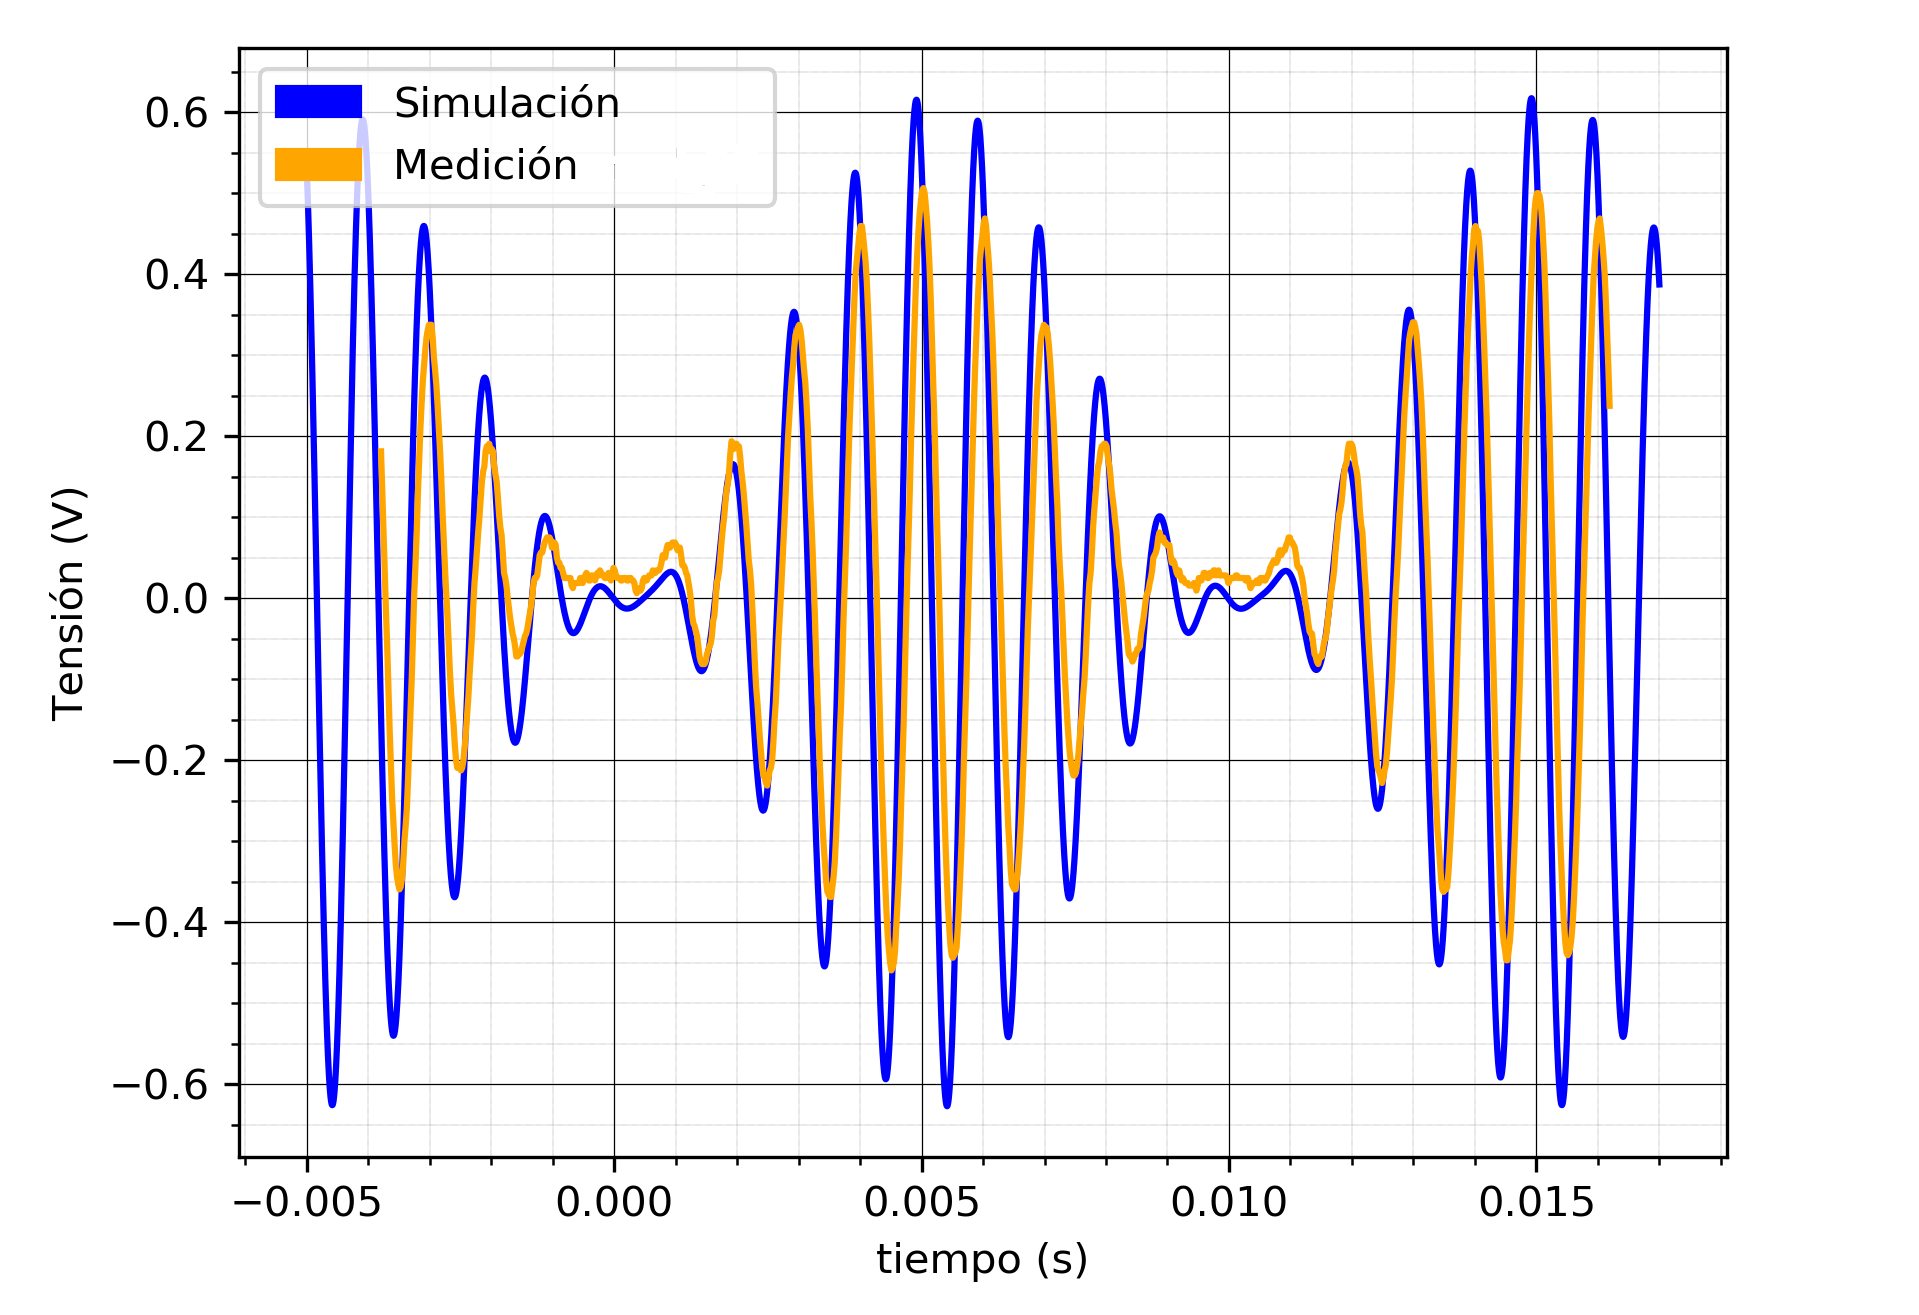
\includegraphics[width=0.7\textwidth]{ej7_meds/med_20.png}
	\caption{Se\~nal AM a la salida del filtro recuperador}
	\label{fig:ej7_out}
\end{figure}

\begin{figure}[htp]
	\centering
	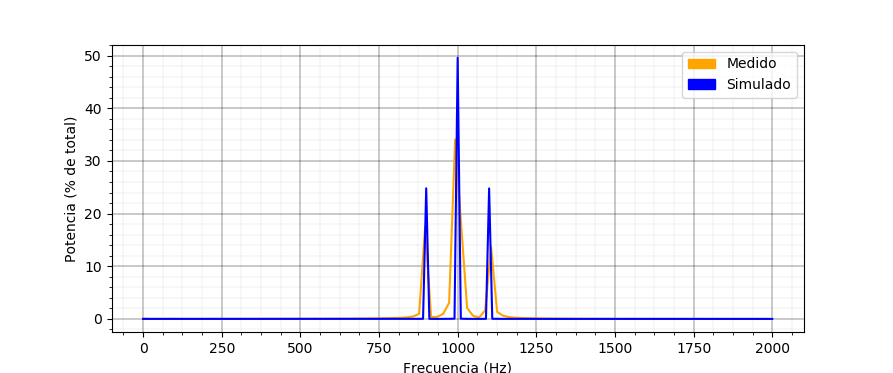
\includegraphics[width=0.7\textwidth]{ej7_meds/7_in.png}
	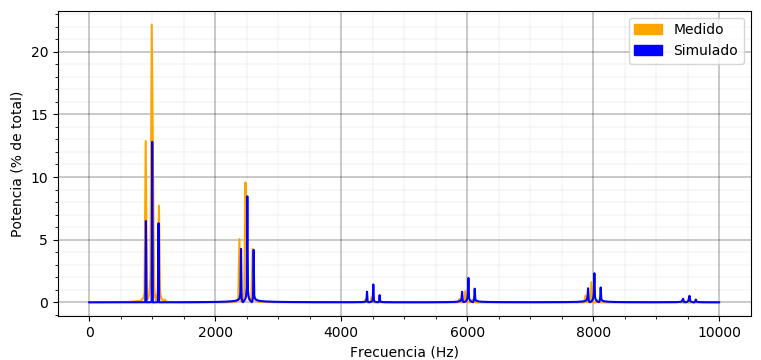
\includegraphics[width=0.7\textwidth]{ej7_meds/7_llave.png}
	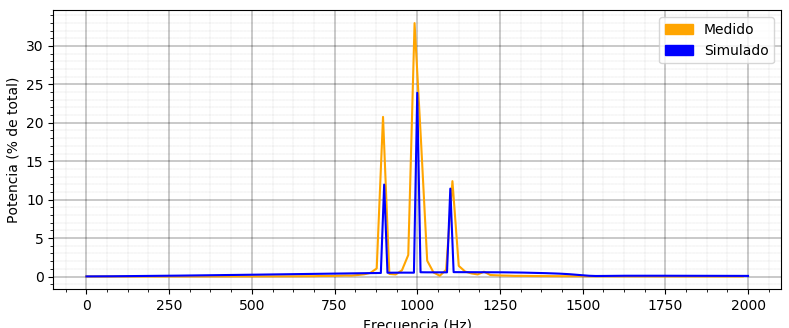
\includegraphics[width=0.7\textwidth]{ej7_meds/7_out.png}
	\caption{Espectros medidos con el analizador de espectro y simulados: entrada (arriba), salida de la llave anal\'ogica (centro), salida }
	\label{fig:ej7_out}
\end{figure}


\end{document}